\documentclass[10pt]{ctexbeamer}
\usepackage[utf8]{inputenc}
\usepackage{xeCJK}
\usepackage{graphicx}
\usepackage {mathtools}
\usepackage{utopia} %font utopia imported
\usetheme{CambridgeUS}
\usecolortheme{dolphin}

% 南邮VI手册给出了南邮指定的颜色代码,
\definecolor{cstd}{cmyk}{100,90,0,0}
\definecolor{cblue}{cmyk}{80,30,0,0}
\definecolor{green}{cmyk}{60,0,100,0}
\definecolor{cyellow}{cmyk}{0,20,100,0}
\definecolor{cblack}{cmyk}{0,0,0,100}
\definecolor{cgrey}{cmyk}{0,0,0,60}
\definecolor{clightgrey}{cmyk}{0,0,0,30}

% 使用转换工具https://www.qtccolor.com/secaiku/tool/convert?m=cmyk将颜色转换为RGB
\definecolor{rstd}{RGB}{2,55,139}
\definecolor{rblue}{RGB}{9,142,202}
\definecolor{rgreen}{RGB}{121,180,28}
\definecolor{ryellow}{RGB}{253,203,0}
\definecolor{rblack}{RGB}{26,23,27}
\definecolor{rgrey}{RGB}{134,135,137}
\definecolor{rlightgrey}{RGB}{197,198,199}


\setbeamercolor*{palette primary}{bg=rgreen}
\setbeamercolor*{palette secondary}{bg=rblue, fg = white}
\setbeamercolor*{palette tertiary}{bg=rstd, fg = white}
\setbeamercolor*{titlelike}{fg=rstd}
\setbeamercolor*{title}{bg=rstd, fg = white}
\setbeamercolor*{item}{fg=rstd}
\setbeamercolor*{caption name}{fg=rstd}
\usefonttheme{professionalfonts}
\usepackage{natbib}
\usepackage{hyperref}
%------------------------------------------------------------
\titlegraphic{
\includegraphics[height=1.5cm]{pic/njupt.logo_full.pdf}}
\logo{
\includegraphics[width=.2\textwidth]{pic/njupt.motto.pdf}}

\setbeamerfont{title}{size=\large}
\setbeamerfont{subtitle}{size=\small}
\setbeamerfont{author}{size=\small}
\setbeamerfont{date}{size=\small}
\setbeamerfont{institute}{size=\small}
\title[南京邮电大学]{现代控制理论的三个月与三十年}
\subtitle{写在人工智能热潮的时代}
\author[李倩茹]{李倩茹 \and 沈梦辰  \and 丕艾谛}

\institute[自动化学院、人工智能学院]{南京邮电大学

自动化学院、人工智能学院}
\date[南京 2022年6月]
{南京 2022年6月}

%------------------------------------------------------------
%This block of commands puts the table of contents at the 
%beginning of each section and highlights the current section:
% \AtBeginSection[]
% {
%  \begin{frame}
%    \frametitle{Contents}
%    \tableofcontents[currentsection]
%  \end{frame}
% }
\AtBeginSection[]{
  \begin{frame}
  \vfill
  \centering
  \begin{beamercolorbox}[sep=8pt,center,shadow=true,rounded=true]{title}
    \usebeamerfont{title}\insertsectionhead\par%
  \end{beamercolorbox}
  \vfill
  \end{frame}
}
%------------------------------------------------------------

\begin{document}

%The next statement creates the title page.
\frame{\titlepage}
\begin{frame}
\frametitle{主要内容}
\tableofcontents
\end{frame}
%------------------------------------------------------------

\section{简介}

\begin{frame}{系统、控制、应用数学}
  控制理论是讲述系统控制科学中具有新观念、新思想的理论研究成果及其在各个领域中,特别是高科技领域中的应用研究成果,但是在民用领域即实际生活中有很严重的脱节。
\end{frame}

\begin{frame}{}
  \begin{enumerate}
    \item 经典控制理论:时域、频域的经典分析与设计(包括基于Nyquist、Bode图的方法,回路整形);根轨迹法;PID控制(Zieglar-Nichols);Wiener滤波;数字控制:Dalin控制,Smith控制,解耦控制,串级控制等;
    \item 现代控制理论:线性系统理论(状态空间法、代数理论、几何理论、多项式频率域方法);最优控制(变分法、极小值原理、动态规划、LQR等);最优状态估计(Kalman滤波、粒子滤波、无迹滤波等);系统辨识(经典与现代方法);自适应控制(模型参考自适应、自校正等);鲁棒控制(H-inf、u、棱边定理等);
    \item 非线性控制理论:非线性系统理论;滑膜变结构;Backstepping等;
  \end{enumerate}
\end{frame}

\begin{frame}{控制一瞥}
  \begin{figure}
    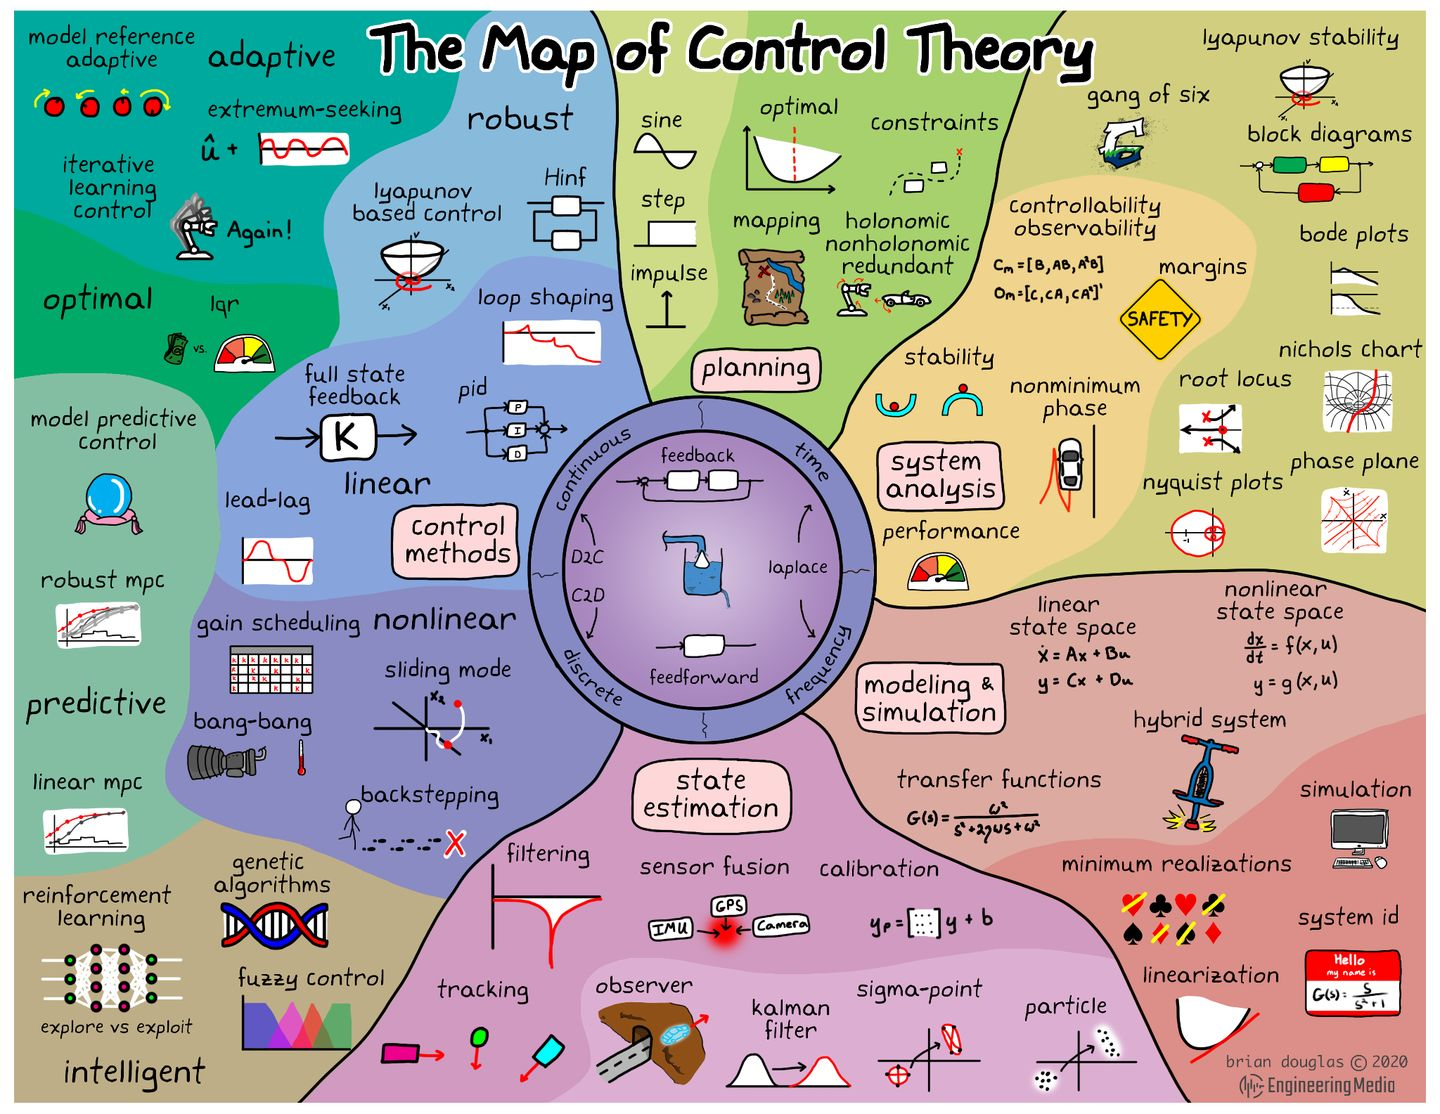
\includegraphics[width=0.8\textwidth]{pic/map_of_control.jpeg}
  \end{figure}
\end{frame}

\section{人工智能}

\begin{frame}{人工智能与控制}
  广义上来讲,机器学习跟控制理论本来就互相包含,比如强化学习(reinforcement learning)本身就起源于最优控制(optimal control),自适应控制(adaptive control)跟在线学习(online learning)以及在线优化(online optimization)息息相关,动态系统里的稳定性(stability)和鲁棒性(robustness)等概念也在机器学习里越来越重要。自动控制(automatic control)最大的目标就是赋予复杂系统“智慧”(full autonomy),这跟人工智能的目标是完全一致的。
\end{frame}

\section{总结与展望}
    \begin{frame}{控制的未来}
    \end{frame}



\section*{致谢}  
  \begin{frame}
  \textcolor{rstd}{\Huge{\centerline{感谢聆听}}}
  \vspace{8pt}
  
  \textcolor{rgreen}{\songti\centerline{感谢各位答辩老师的聆听,恳请老师批评指正}}
  \end{frame}

\end{document}